%----------------------------------------------------------------------------------------
%	PACKAGES AND THEMES
%----------------------------------------------------------------------------------------

\documentclass{beamer}

\mode<presentation> {

% The Beamer class comes with a number of default slide themes
% which change the colors and layouts of slides. Below this is a list
% of all the themes, uncomment each in turn to see what they look like.

%\usetheme{default}
%\usetheme{AnnArbor}
%\usetheme{Antibes}
%\usetheme{Bergen}
%\usetheme{Berkeley}
%\usetheme{Berlin}
%\usetheme{Boadilla}
%\usetheme{CambridgeUS}
%\usetheme{Copenhagen}
%\usetheme{Darmstadt}
%\usetheme{Dresden}
%\usetheme{Frankfurt}
%\usetheme{Goettingen}
%\usetheme{Hannover}
%\usetheme{Ilmenau}
%\usetheme{JuanLesPins}
%\usetheme{Luebeck}
\usetheme{Madrid}
%\usetheme{Malmoe}
%\usetheme{Marburg}
%\usetheme{Montpellier}
%\usetheme{PaloAlto}
%\usetheme{Pittsburgh}
%\usetheme{Rochester}
%\usetheme{Singapore}
%\usetheme{Szeged}
%\usetheme{Warsaw}

% As well as themes, the Beamer class has a number of color themes
% for any slide theme. Uncomment each of these in turn to see how it
% changes the colors of your current slide theme.

%\usecolortheme{albatross}
%\usecolortheme{beaver}
%\usecolortheme{beetle}
%\usecolortheme{crane}
%\usecolortheme{dolphin}
%\usecolortheme{dove}
%\usecolortheme{fly}
%\usecolortheme{lily}
%\usecolortheme{orchid}
%\usecolortheme{rose}
%\usecolortheme{seagull}
%\usecolortheme{seahorse}
%\usecolortheme{whale}
%\usecolortheme{wolverine}

%\setbeamertemplate{footline} % To remove the footer line in all slides uncomment this line
%\setbeamertemplate{footline}[page number] % To replace the footer line in all slides with a simple slide count uncomment this line

%\setbeamertemplate{navigation symbols}{} % To remove the navigation symbols from the bottom of all slides uncomment this line
}

\usepackage{graphicx} % Allows including images
\usepackage{booktabs} % Allows the use of \toprule, \midrule and \bottomrule in tables

\usepackage{lmodern}% http://ctan.org/pkg/lm
% Allows arbitrary font size
% https://tex.stackexchange.com/questions/58087/how-to-remove-the-warnings-font-shape-ot1-cmss-m-n-in-size-4-not-available

\usepackage{array, amsmath, amssymb, amsfonts} % math typesetting
\usepackage{tabularx, booktabs, multicol, multirow, longtable} % tables

\usepackage{verbatim, listings} % paste code in latex
\lstset{
	language=R,
	basicstyle=\scriptsize\ttfamily,
	 commentstyle=\ttfamily\color{gray},
	numbers=left,
	 numberstyle=\ttfamily\color{gray}\footnotesize,
	stepnumber=1,
	numbersep=5pt,
	backgroundcolor=\color{white},
	showspaces=false,
	showstringspaces=false,
	showtabs=false,
	frame=single,
	tabsize=2,
	captionpos=b,
	breaklines=true,
	breakatwhitespace=false,
	title=\lstname,
	escapeinside={},
	keywordstyle={},
	morekeywords={}
	}
%----------------------------------------------------------------------------------------
%	TITLE PAGE
%----------------------------------------------------------------------------------------

\title[Conflict Prediction]{Conflict Prediction and Machine Learning} % The short title appears at the bottom of every slide, the full title is only on the title page

\author{Anh Le} % Your name
\institute[Duke] % Your institution as it will appear on the bottom of every slide, may be shorthand to save space
{
Duke University \\ % Your institution for the title page
\medskip
\textit{anh.le@duke.edu} % Your email address
}
\date{\today} % Date, can be changed to a custom date

\begin{document}

\begin{frame}
\titlepage % Print the title page as the first slide
\end{frame}

\begin{frame}
\frametitle{Overview} % Table of contents slide, comment this block out to remove it
\tableofcontents % Throughout your presentation, if you choose to use \section{} and \subsection{} commands, these will automatically be printed on this slide as an overview of your presentation
\end{frame}

%----------------------------------------------------------------------------------------
%	PRESENTATION SLIDES
%----------------------------------------------------------------------------------------

\begin{frame}
\frametitle{Spike and Slab model}

\begin{figure}
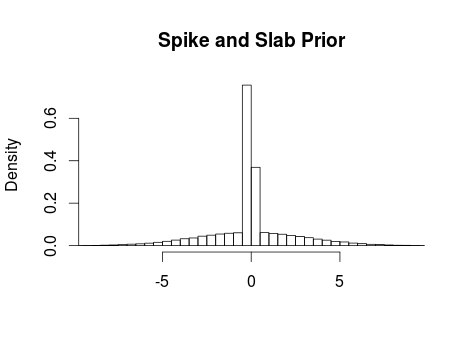
\includegraphics[width=\textwidth]{../image/spike_and_slab}
\end{figure}
\end{frame}

%------------------------------------------------


%------------------------------------------------

\begin{frame}
\frametitle{Model performance (with country dummies)}
\begin{table}[H]
\centering
	% latex table generated in R 3.1.2 by xtable 1.7-4 package
% Mon Dec  8 12:02:52 2014
\begin{tabular}{rrrrrr}
  \hline
 & insurgency & rebellion & dpc & erv & mp \\ 
  \hline
brier & 0.080 & 0.057 & 0.167 & 0.037 & 0.049 \\ 
  auc.C & 0.886 & 0.895 & 0.688 & 0.922 & 0.704 \\ 
  precision & 0.519 & 0.575 & 0.162 & 0.508 & 0.097 \\ 
  recall & 0.778 & 0.586 & 0.458 & 0.504 & 0.033 \\ 
   \hline
\end{tabular}

	\caption{Spike and Slab (out-sample)}
\end{table}
\begin{table}
	\begin{tabular}{rrrrr}
  \hline
 & insurgency & rebellion & dpc & erv \\ 
  \hline
brier & 0.06 & 0.03 & 0.12 & 0.03 \\ 
  auc.C & 0.94 & 0.97 & 0.78 & 0.93 \\ 
   \hline
\end{tabular}
	\caption{EBMA (out-sample)}
\end{table}
\end{frame}

\begin{frame}
\frametitle{Variable selection (rebellion)}
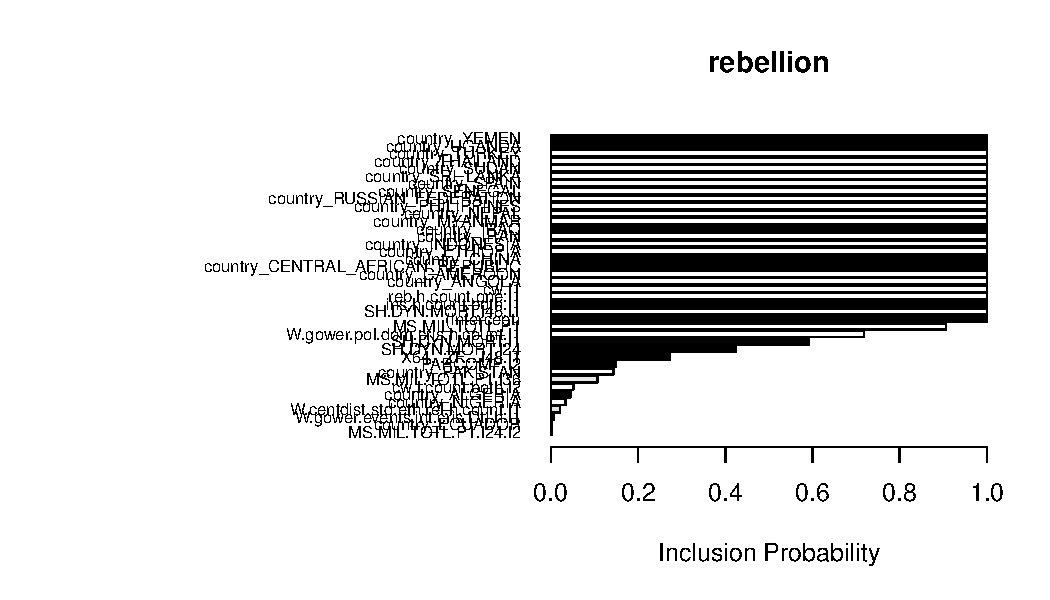
\includegraphics[width=\textwidth]{fig/spikeslab_rebellionvar}
\end{frame}

\begin{frame}
\frametitle{Model performance (without country dummies)}

\begin{table}[H]
	% latex table generated in R 3.1.2 by xtable 1.7-4 package
% Mon Dec  8 12:02:52 2014
\begin{tabular}{rrrrrr}
  \hline
 & insurgency & rebellion & dpc & erv & mp \\ 
  \hline
brier & 0.080 & 0.057 & 0.167 & 0.037 & 0.049 \\ 
  auc.C & 0.886 & 0.895 & 0.688 & 0.922 & 0.704 \\ 
  precision & 0.519 & 0.575 & 0.162 & 0.508 & 0.097 \\ 
  recall & 0.778 & 0.586 & 0.458 & 0.504 & 0.033 \\ 
   \hline
\end{tabular}

	\caption{With dummies (out-sample)}
\end{table}

\begin{table}
	% latex table generated in R 3.1.2 by xtable 1.7-4 package
% Mon Dec  8 18:36:13 2014
\begin{tabular}{rrrrrr}
  \hline
 & insurgency & rebellion & dpc & erv & mp \\ 
  \hline
brier & 0.080 & 0.057 & 0.167 & 0.037 & 0.049 \\ 
  auc.C & 0.886 & 0.895 & 0.688 & 0.922 & 0.704 \\ 
  precision & 0.519 & 0.575 & 0.162 & 0.508 & 0.097 \\ 
  recall & 0.778 & 0.586 & 0.458 & 0.504 & 0.033 \\ 
   \hline
\end{tabular}

	\caption{Without dummies (out-sample)}
\end{table}
\end{frame}

\begin{frame}
\frametitle{Boosted classification tree}
\begin{itemize}
\item Fit an initial tree
\item Get the residuals, fit another tree to the residual
\item Add (part of)the new tree to the existing tree
\item Tune 1) the number of trees, 2) how much of the new tree to add back to the old tree, 3) the complexity of each tree
\end{itemize}

So the algorithm can learn \textit{slowly}
\end{frame}

\begin{frame}
\frametitle{Boosted tree result (for 2-month out...)}
\begin{table}
	% latex table generated in R 3.1.2 by xtable 1.7-4 package
% Wed Feb 11 15:42:07 2015
\begin{tabular}{rrrrrr}
  \hline
 & insurgency & rebellion & dpc & erv & mp \\ 
  \hline
brier & 0.006 & 0.005 & 0.039 & 0.031 & 0.033 \\ 
  auc.C & 0.997 & 0.999 & 0.946 & 0.980 & 0.857 \\ 
  precision & 0.971 & 0.965 & 0.705 & 0.542 & 0.541 \\ 
  recall & 0.964 & 0.968 & 0.521 & 0.926 & 0.118 \\ 
   \hline
\end{tabular}

	\caption{Boosted tree (in-sample)}
\end{table}
\begin{table}
	% latex table generated in R 3.1.1 by xtable 1.7-3 package
% Sun Jan 25 23:20:49 2015
\begin{tabular}{rrrrr}
  \hline
 & insurgency & rebellion & dpc & erv \\ 
  \hline
brier & 0.008 & 0.012 & 0.091 & 0.037 \\ 
  auc.C & 0.996 & 0.984 & 0.899 & 0.956 \\ 
  precision & 0.971 & 0.958 & 0.584 & 0.659 \\ 
  recall & 0.963 & 0.854 & 0.730 & 0.712 \\ 
   \hline
\end{tabular}

	\caption{Boosted tree (out-sample)}
\end{table}

\end{frame}

\end{document} 